% English translation of capitulos/05-discussao.tex, made by Claude Code (Claude Fable 5.2) on 24 November 2026.
% Pending review by the author. When the Portuguese file changes, update this one (scripts/verificar_traducao.py).
\section{Discussion and Application}\label{sec:discussao}
This section interprets the results of Section~\ref{sec:resultados} and presents the application that makes them available for
public consultation (Section~\ref{sec:aplicacao}). The interpretations are those of this work and
depend on records extracted by AI and checked by the author only in a sample.

\subsection{What the results indicate}
\textit{The evidence is mostly about packages.} Most of the focal techniques were evaluated as a complete system
against a baseline, and the gain of a package does not tell which mechanism produced it. Component ablations
exist in 191 studies, but they isolate ingredients within the system of each study, in general with few models and
benchmarks. For this reason, the taxonomy by mechanism describes what is evaluated more safely than
how much each mechanism contributes.

\textit{The call budget is a recurring confounding factor.} The iterative, multi-agent and
sampling packages use more calls and more tokens than the baselines. In the conditions extracted from the two studies that equalize the
budget of attempts, the feedback loop did not outperform sampling without repair (S479-C2; S645-C1).
% AFIRMACAO: A63
One possible reading is that part of the gains attributed to iteration accompanies the increase in attempts. This
hypothesis was not tested here and deserves studies that equalize the budget.
% AFIRMACAO: A69

\textit{The size of the model and the origin of the intermediate content condition the sign.} The reasoning instruction
had a mixed result when added to the prompt, with no significant effect in one study and drops with small
models or with a generation limit (S560-C2; S1121-C1; S1606-C4).
% AFIRMACAO: A74
% AFIRMACAO: A75
When the reasoning or the plan came from another model, stronger or fine-tuned, the result improved. In that case, the
effect is confounded with the choice of the model (S1121-C4; S216-C1). Self-correction without execution also got worse with a
1.5B model (S759-C1).
% AFIRMACAO: A68
In repair, explicit reasoning got worse in almost all the extracted comparisons.

\textit{Verifiable external information appears in a good part of the favourable results.} Many of the favourable
contrasts come from conditions that bring new information to the model: tests, execution, repository context and
localization of the defect, under the conditions of each study. Since models, metrics and benchmarks differ, this
does not establish that this information outperforms instructions in general. Part of them, however, uses oracle information, taken from the reference solution, and indicates an upper
bound, and not realistic use (S670-C5).
% AFIRMACAO: A84
Changes only in wording, persona or language of the instruction had small, null or negative effects. More
context is also not always better: there were drops with inadequate retrieval (S806-C1) and with bulky context
in repair.
% AFIRMACAO: A85

\textit{Non-functional requirements bring trade-offs.} Security instructions reduced vulnerabilities in some
studies and reduced functional correctness in others (S1195-C4). The measurement of these trade-offs is rare, and the
scanners used do not demonstrate security in real use.
% AFIRMACAO: A87

\textit{Translation and refactoring have little evidence.} In translation, compilation and test feedback
appears favourable in packages, but the ablation of one study attributes most of the difference to the tests in the prompt
(S329-C2; S329-C3).
% AFIRMACAO: A27
Explaining before translating did not improve the result (S193-C1).
% AFIRMACAO: A30
In refactoring, specifying the type of transformation or providing API knowledge brought the largest gains, from low baselines and in few studies (S511-C2; S2122-C1).
% AFIRMACAO: A37

\subsection{Implications for the choice of techniques}
The decision-support table (Table~\ref{tab:apoio}) guides by conditions, and not by winning techniques. It suggests three
questions for those choosing a technique:
\begin{itemize}
  \item are there tests, an executor or a compiler to provide feedback?
  \item what is the budget of calls and of tokens?
  \item is the model small or large?
\end{itemize}
Where the evidence is mixed, as in the reasoning instruction, in self-critique without execution, in the fixed
repair examples and in the security instructions, the guidance is to test locally before adopting, and not to recommend the technique
as a default. In the examination in eight scenarios (Section~\ref{sec:exame}), the table led
to an executable script only when the condition of the scenario coincided with that of the studies, and version 2,
revised after the examination, declares insufficient evidence and the result measured. The examination verifies clarity, grounding and concreteness,
but not effectiveness.

\subsection{Application: the Prompt em Código system}\label{sec:aplicacao}
% Section included on 22 November 2026 at the suggestion of the advisor (D137). It describes the system published
% on 21 November 2026 (D131 and D132); it brings no new empirical claims about the studies.
% Local \emergencystretch: allows the line to break before or inside the address without invading the margin.
{\emergencystretch=4em
The decision-support table and the extracted comparisons were published in an open-access web system, Prompt em
Código, available at \url{https://caiofreitas1.github.io/tcc2-prompt-engineering/}. The system was developed in
November 2026, after the presentation of the work to the examining committee, which asked for the research
results to be made available in a system open to the public. It runs in the browser, requires no registration and does not send
to the server the conditions entered by the user. The data come from a single file, generated from version 2
of the decision-support table (Tables~\ref{tab:apoio} and~\ref{tab:apoiob}), from the 332 records and from the 805 comparisons. The system
publishes values, locators and addresses of the sources, without reproducing passages of the articles. It has three screens:
Guide, Explorer and About.\par}

The Guide applies the questions of the previous section to the 31 rows of the table. Its use follows four steps:
\begin{enumerate}
  \item choose the task: generation, debugging, translation or refactoring;
  \item tick the resources available, which are executable tests, code executor, compiler, static
  analyser, repository or documentation to retrieve context, examples and a small model run locally, and
  state whether it is possible to make one or several calls to the model; in debugging, also state whether the defect can
  be reproduced and whether there is a message, output or report of the defect;
  \item read the rows of the task, which the system separates into three groups: applicable to the conditions ticked, rows that
  require a resource not ticked and declared gaps;
  \item open a row to see the condition studied, the result measured, the indication, the strength of the evidence, the
  caveats and the comparisons cited, each with the two values, the model, the benchmark, the metric and the
  location of the result in the source.
\end{enumerate}
It is also possible to start from one of the eight scenarios of the examination (Section~\ref{sec:exame}), which fill in the conditions; they
can be changed afterwards. In scenario G1, for example, the Guide shows the 14 generation rows: 8 applicable, 3
that require a resource not ticked and 3 gaps (Figure~\ref{fig:guia}).

\begin{figure*}[!htb]
\centering
% In the monograph (ABNT), the caption goes above the figure; in the article, below.
\ifdefined\fontetabela\caption{Guide screen with the conditions of scenario G1, on 22 November 2026}\label{fig:guia}\fi
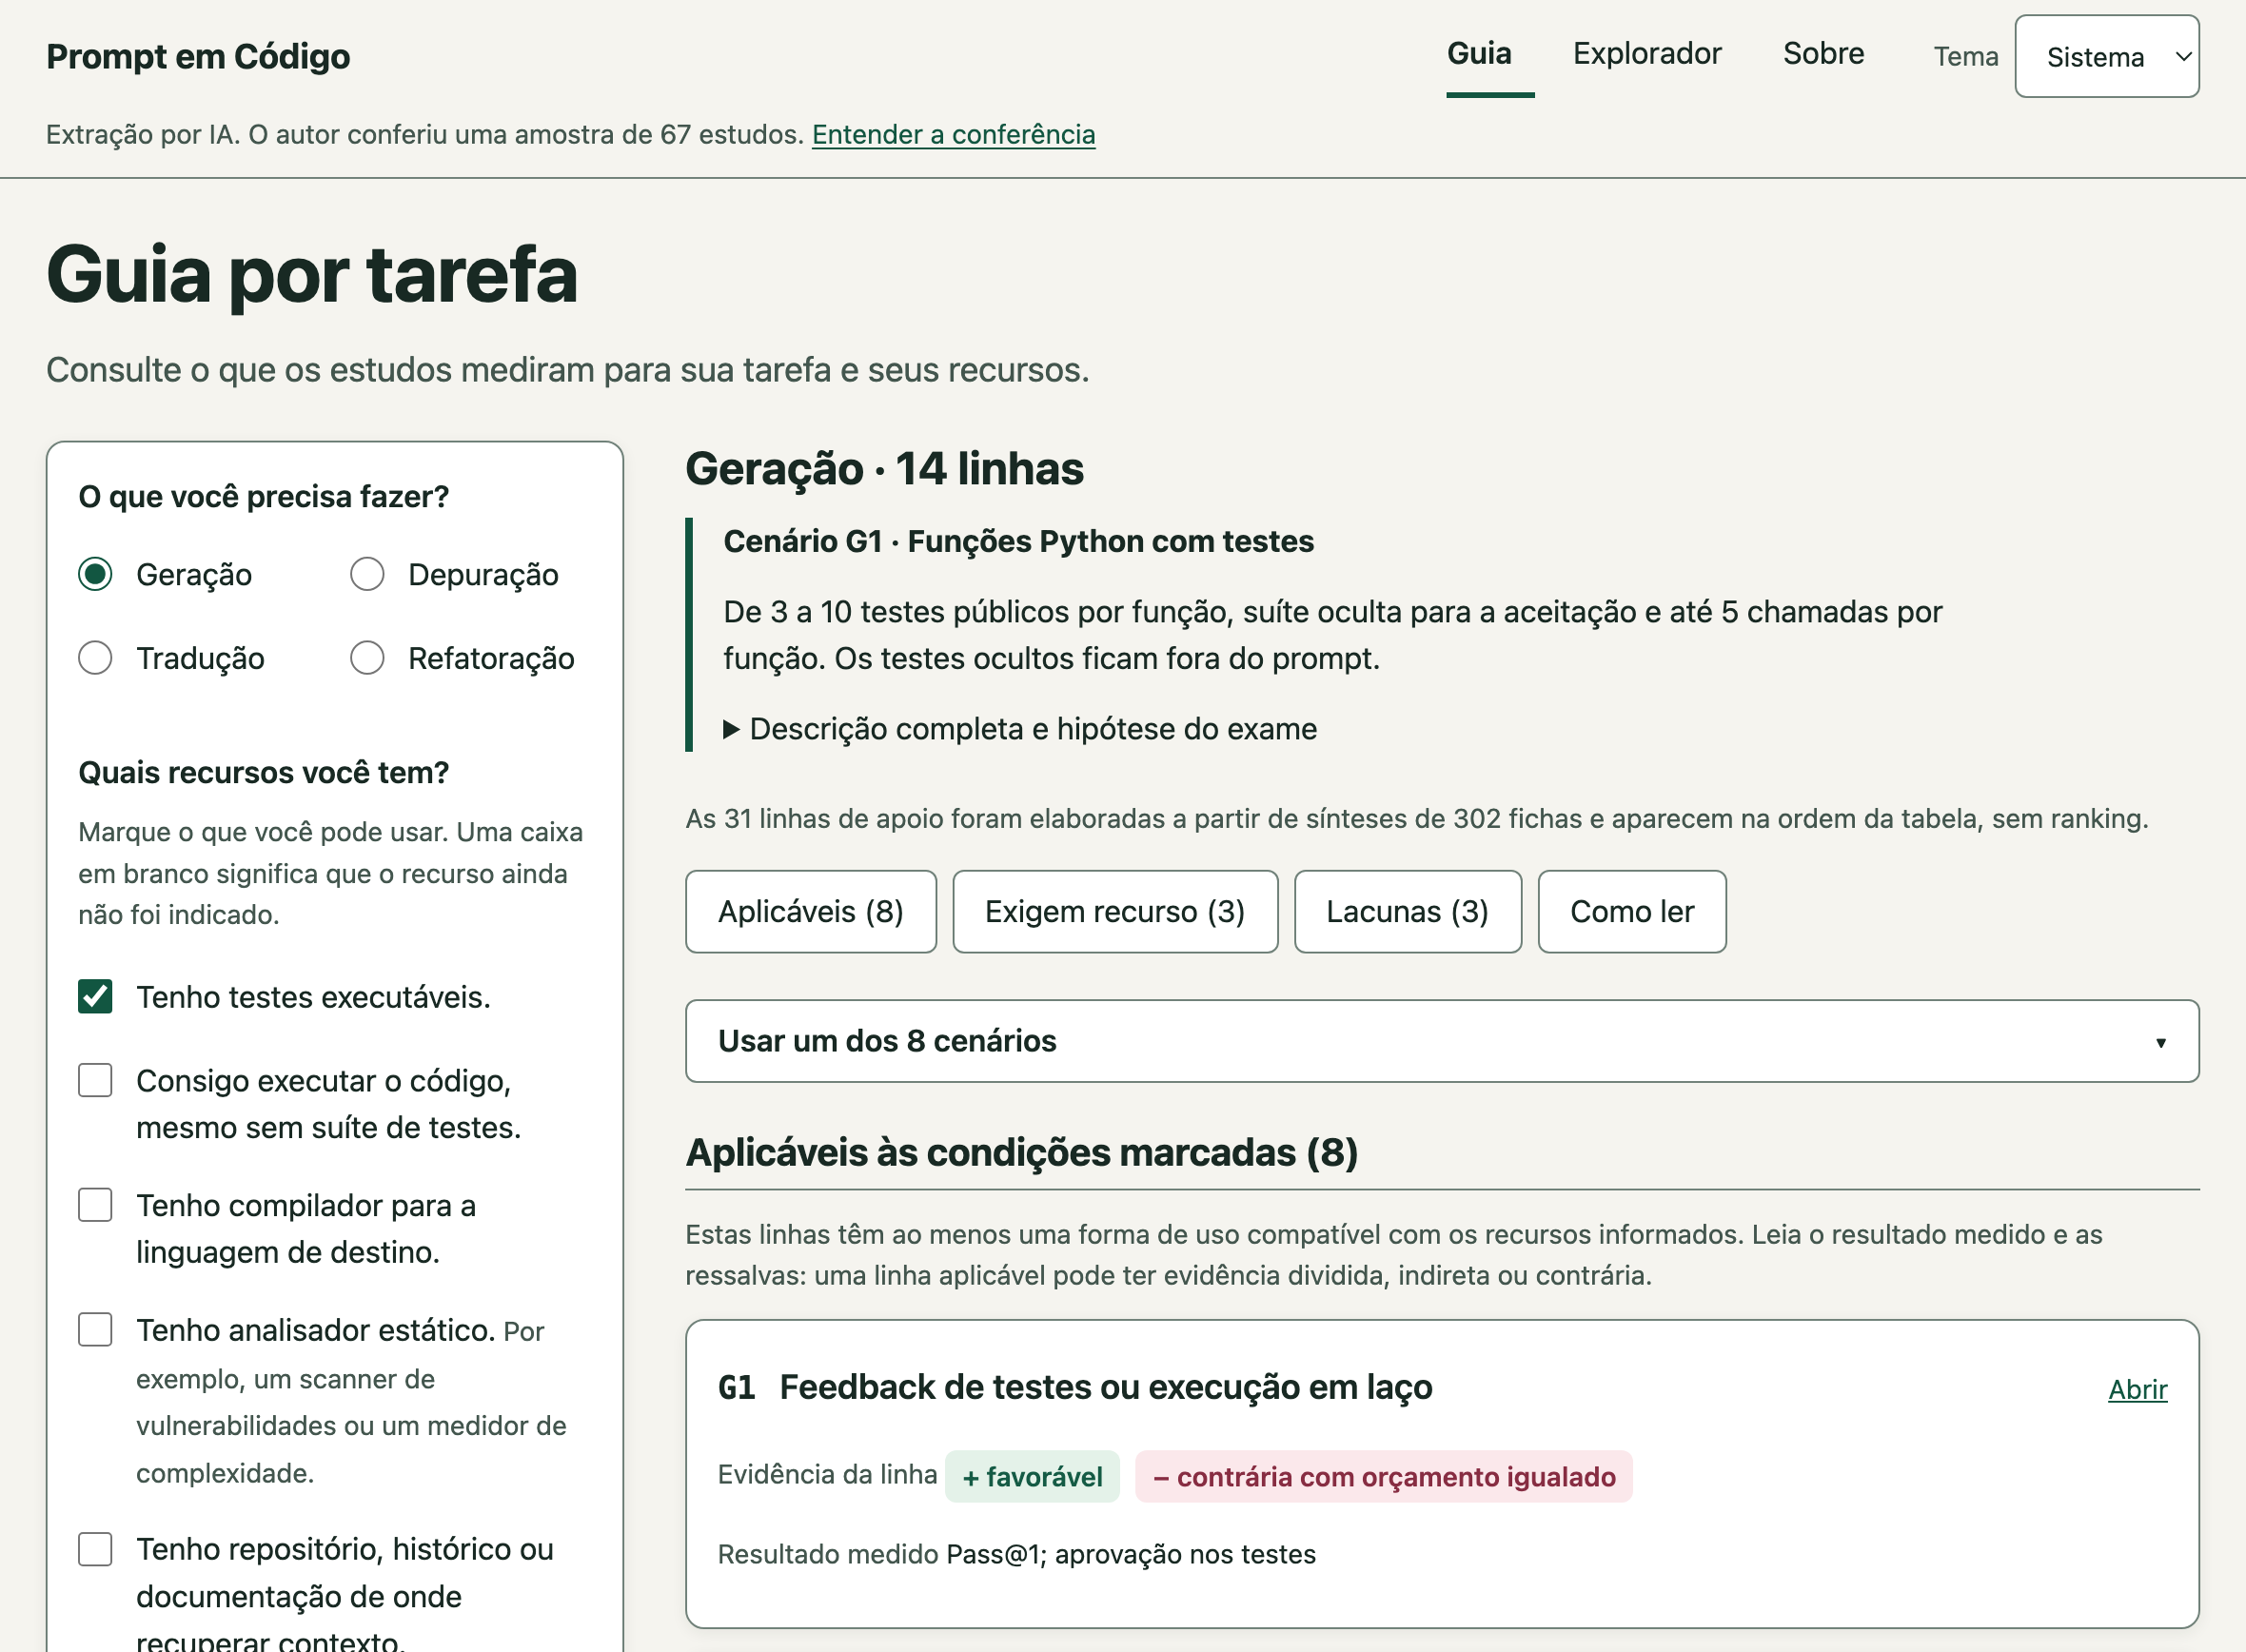
\includegraphics[width=\textwidth,height=0.42\textheight,keepaspectratio]{figuras/guia-cenario-g1}
\ifdefined\fontetabela\else\caption{Guide screen with the conditions of scenario G1, on 22 November 2026 (interface in Portuguese)}\label{fig:guia}\fi
\end{figure*}

The Explorer gives access to the 805 comparisons. The search looks up identifier, study title, technique,
comparator, model, benchmark and metric, and the filters select task, mechanism added and direction
of the comparison. A matrix shows the count of comparisons per mechanism added and task, and each cell opens
the corresponding list. The index of studies leads to the record of each of the 332 studies, with its techniques, its
comparisons and the address of the source, when recorded. The About screen summarizes the method, explains how to read the terms used and reports the
coverage of the data and the status of the check.

The system keeps the limits of the synthesis. The rows appear in the order of the table, without ranking and without averaging
across benchmarks, and each pair of values is presented separately. An applicable row is one whose
required resources were ticked, and its evidence may be mixed, indirect or contrary. Each comparison
states that the extraction was made by AI and whether it belongs to the sample checked by the author. The rows of the Guide come from the
syntheses of 302 records, and the later extractions appear only in the Explorer. The separation of the rows into the three
groups and the filling in of the scenarios were derived from the condition column of the table, with AI support, and do not yet
have a recorded review by the author. They are editorial decisions of the system, and not results of the review.

The design specification was made by Codex and the implementation, by Claude Code, AI assistants, at the request of the
author. The code, the data and the automated tests that compare the published file with the sources are in the
project repository. The verification consisted of these tests and of the inspection of the screens in the browser. The system was not
evaluated with users, and for this reason this work does not claim its usefulness or its usability.

\subsection{Comparison with other reviews}\label{sec:comparacao}
The general reviews of LLMs in software engineering describe which prompting techniques the studies use, but not
what each one adds to the prompt or under which condition it works. \citet{hou2024slr} count the frequency
of the techniques in studies up to January 2024. This work covers only four tasks, includes studies up to 2026 and
records, per comparison, the type of counterfactual, the direction and the conditions. This explains the main difference in
reading: most of the evidence is of packages against baselines, which a usage count does not show.

Two points converge with closely related reviews.
The role of verifiable external information, such as tests, execution and repository context, in the favourable
results of this corpus is consistent with the emphasis of \citet{fan2023survey} on hybrid techniques, which
combine traditional software engineering and LLMs.
% AFIRMACAO: A120
The dependence on perfect localization of the defect, recorded here in the debugging rows, also appears in
\citet{yang2025aprsurvey}, who record this assumption for each repair system, because it makes the
results hardly comparable across articles.
% AFIRMACAO: A122
On energy efficiency, \citet{masthanali2026energy} did not find a prompting strategy
that improves the result consistently, which resembles the mixed results of the instructions and of
self-critique without execution in this work.
% AFIRMACAO: A123

The reviews of prompting techniques, such as that of \citet{sahoo2024survey}, organize the techniques by area
and summarize the results reported by their authors, without crossing them with the evaluation conditions. The decision-support table
of this work tries to fill this gap for the four tasks, with the caveat that the search was not designed
to locate reviews and, therefore, no claim is made that the combination is new.

\subsection{Threats to validity}\label{sec:ameacas}
The threats below follow from the method carried out up to 17 November 2026.

\textit{Search coverage.} The search used three databases and a single search string, applied to title and abstract. The string
did not retrieve two of the six studies of the reference set (S3 and S5), because title and abstract do not combine the
three blocks of terms, which indicates a potential coverage limitation; the eligibility of these two studies was not
assessed. There was no broad snowballing to compensate.
The number of studies retrieved does not, by itself, demonstrate that the coverage is adequate.

\textit{Concessions of the rapid review.} Requiring the task in the title reduced the candidates from 2,304 to 715, but, in the
calibration samples, 46 of the 79 studies included by the author (58\%) did not have the task in the title and would be left
out (Section~\ref{sec:calibracao}). This is the main limitation of the work: the corpus represents the studies that
name the task in the title, and not the whole literature on the subject. The cut of stage 2 removes 233 studies available
only on arXiv, which tends to under-represent the most recent work, still without a reviewed publication.

\textit{Access to the texts.} The protocol started restricted to open access and came to accept the institutional access
of UFMG after the title and abstract screening. Studies outside the two types of access are not read. Stage 3,
almost all from IEEE Xplore, was read by the models and checked by the author in the 111 studies. IEEE Xplore studies
without institutional access and those only on arXiv (stage 2) remain outside the corpus of this version.

\textit{AI-assisted selection.} The screening was done by two models from the same vendor (Claude Opus 5.5 and Claude
Sonnet 5.5), which may err in the same way. For this reason, the agreement between them ($\kappa = 0.726$ at title and
abstract and $\kappa = 0.745$ in the 419 full-text studies) does not indicate correctness. The comparison with the author shows
relevant disagreements: at full text, with the author's first decision, $\kappa = 0.641$ with AI-A and
$0.548$ with AI-B. Of the 60 consensual exclusions at
full text, the author included 5, and, at title and abstract, 7 of the 92. Since the author checked all the consensual
exclusions in the two phases, these studies were not lost. The measure, however, shows that exclusion by two
models does not dispense with the human check. There is a single human reviewer, and not independent dual human
screening.

\textit{Application of the criteria.} The rule of I2 for the full text was defined after the calibration, and the boundary of
X4 for studies in which prompting is only a baseline was formulated during the check. Both were decided
in view of the data and may reflect the cases that motivated them. The boundary of X4 depends on judging whether a prompting result is
analysed as a finding or serves only as a reference, and this judgement may vary between readers; with a single
human reviewer, this variation was not measured. The boundary was applied to S314 and S373 on the basis of the reasons already
recorded, without a new reading. Of the nine studies in doubt, eight were excluded later, and one (S1617) was included by the
rule of the date of the event.

\textit{Reading from the extracted text.} The models read the text extracted from the PDFs, without figures and with tables sometimes
scrambled, returning to the PDF only in case of doubt. In three studies, one of the models read only part of the text, and
in seven long texts it was not verified whether the reading was complete. The author read all the 419 studies checked, which reduces,
but does not eliminate, the effect of these failures on the selection.

\textit{Extraction and synthesis.} The extraction was done by AI, with a single extractor per study. Two models
worked on the 332 records: Claude Opus 5.5 on 295 studies and Codex on 27, plus the 10 pilot records,
extracted by Opus. The calibration in the pilot
showed errors in reading values and in selecting comparisons, and does not estimate the error rate in new studies. The author checked the 67
studies of the sample after the synthesis and corrected 18 of 571 blocks (3.2\%), but 56 of these studies have only the
declaration that they were correct, without a record per block. The rate holds for the blocks judged; outside the sample, the records remain
as extraction by AI. The synthesis by grouping was drafted in a first
version by subagents, over excerpts of the records. The automatic check confirmed that the identifiers
cited exist, but not that each sentence reflects the study. The author checked each claim
against the original and marked 30 of the 120 for correction. The limit of three comparisons per study, chosen without looking at the effect, reduces selective choice in the
extraction, but leaves out results that the authors report in other tables. The heterogeneity recorded in a
targeted search compensates only in part for this loss. The studies use different models, benchmarks and
metrics, and for this reason the synthesis does not compute averages or rank techniques. Results on benchmarks do not,
by themselves, demonstrate gains in productivity, security or cost. They may be affected by contamination of the
training data, which 187 of the 332 studies with a record do not address.

\textit{Validation of the practical contribution.} The taxonomy and the decision-support table were examined in eight synthetic
scenarios, with judgement by the author, without external users or an experiment. This examination verifies clarity, grounding in the sources and concrete guidance, but
does not measure the effectiveness of the techniques or the usefulness of the table for developers. The system of
Section~\ref{sec:aplicacao} was also not evaluated with users.

\subsection{Social, economic and environmental impacts}
The studies of the corpus measure performance on benchmarks and, in few cases, cost or energy. The evidence on
the performance of developers is scarce: S62 measures time and accuracy of 20 participants in a delimited task of
reviewing patches, with and without explanations, with no significant difference in time (S62, section 5.4). These
results do not allow general productivity gains to be concluded, and for this reason this work does not claim economic
gains.

Among the impacts measured, multi-step techniques multiply calls and tokens. MapCoder, for
example, used on average 16.7 calls and 21.25 thousand tokens, against one call and 0.64 thousand tokens for the
direct prompt (S344).
% AFIRMACAO: A57
This cost also has an environmental dimension, since repair consumed from 5 to 15 times the energy of the single pass in
one study (S1415). Risks to the security of the code were also measured, such as the vulnerabilities introduced
or preserved in translation (S951) and those accumulated in improvement iterations (S739).
% AFIRMACAO: A50

The effects on those who use the techniques hardly appear in the records. One exception is the report of participants who
accepted without scrutiny the reasoning of incorrect patches (S62).
% AFIRMACAO: A60
This type of effect calls for more studies with users; the few present in the corpus, such as that of S62, cover delimited
tasks.
